\documentclass[a4paper,12pt]{article}
\usepackage[hidelinks]{hyperref}
\usepackage{graphicx}
\usepackage{float}
\usepackage{caption}
\begin{document}
\begin{center}

%Cover page
\Huge\textbf{User Manual(uWatch digital forensic tool)\\}
																											
\vspace{2 cm}
Affiliation with SAPS and ICSA(Ms. S.Omeleze and Prof. H.Venter)\newline 
\vspace{2 cm}
\LARGE\textbf{Creators:} MPHETamines
\begin{tabular}{lr}
Taariq Ghoord&10132806
\\
Phethile Mkhabela&12097561
\\
Sboniso Masilela&10416260
\\ 
Martha Mohlala&10353403
\\
Harrison Maphuti Setati&12310043\\
\end{tabular}

\vspace{1cm}
\textbf{Git repository link:\\}
\url{https://github.com/MPHETamines/MPHETamines/}

\vspace{1cm}
\textbf{Date:} 04 August 2015
\end{center}
\pagenumbering{gobble}
\newpage

%table of contents
\tableofcontents

\newpage
\pagenumbering{arabic}

\section{General Information}
\subsection{System Overview}
This system is intended for those who wish to help a community of overgrowing crime with no prosecution. The application assists users in capturing evidence and making that evidence readily available to the court of law. Anybody may use the application in order to clean our streets up by making prosecution easy by means of genuine digital evidence. The police enforcement and court of law will both be able to access the system to use the evidence provided by the citizens of South Africa.

\subsection{System Configuration}
The equipment for the use of the system is just a smart device with access to the internet, the application supports all major platforms so IOS, Android or Windows mobile will do, The devices should also be able to capture video and images as well as have an audio recorder as most devices do now-days. The court will access the evidence from any device with a web browser and all the evidence is stored on a cloud server. To configure ones device to effectively use the application we advise to have a good internet access, location switched on, and high quality image and video capture settings in the camera. To effectively use the court system web view of evidence a strong internet connection is required.

So the process is as follows, The users device uploads the evidence captured by the user to a cloud and from there the court system can view the evidence by downloading it from the cloud, the court can see who uploaded the evidence, when it was uploaded, where the incident took place, as well as any tags associated with the incident.

\subsection{Installation}
The software will be available on all platforms app markets available for download. This includes IOS, Android and Windows mobile. To install one would just need to search the app market for uWatch and select install then accept the agreements. After this the application will be installed to the device. 

\section{Getting started}
For the average citizen using the application to capture evidence, one would need to register an account which is an easy procedure done in the application. After registering the user will be prompted to login with the account he/she has just created. An email address is required to register. Changing user names is not allowed in the application but changing a password will be available by simply clicking the forgot password link and then following the emails in order to reset ones password. When logged in the user can either view the evidence previously captured or capture new evidence. Evidence can either be a voice recording, video clip, or image. After capturing the user can decide to discard or send the evidence to the server where it will be securely stored. The user may also associate tags to the evidence just captured. 
\section{Using the system}
\subsection{Opening uWatch}
After you have downloaded uWatch from app store,click on the app and the splash screen that looks like the image below will popup and lead you to the login screen.
\begin{figure}[H]
\begin{center}

\includegraphics[width=50mm,scale=0.5]{images/screenshots/splashscreen.png}
\end{center}
\end{figure}
\subsection{Registering}
You can either capture the digital evidence first by clicking on the capture tab shown on the top bar of the screen below or login first.If you are the new user you need to register before logging in.
\begin{figure}[H]
\begin{center}
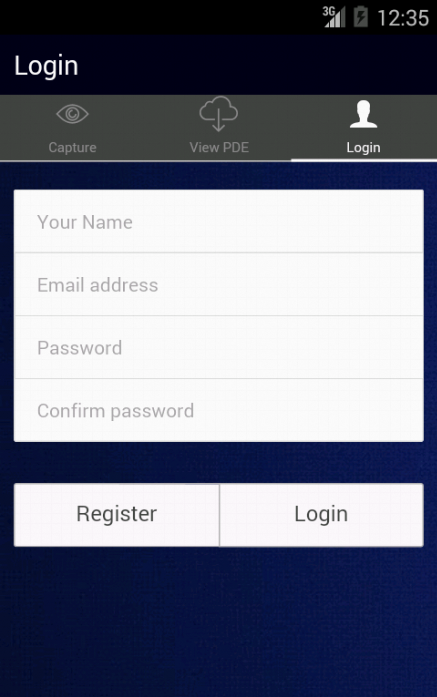
\includegraphics[width=50mm,scale=0.5]{images/screenshots/register.png}
\end{center}
\end{figure}
\subsection{Login}
The screen below is a login screen where you are required to put your email address as your username, and a password.If your username or password is incorrect, the next screen will pop up as alert. Please retry to login with correct credentials if you are a registered user. If you are not registered user please try to register before logging in.
\begin{figure}[H]
\begin{center}
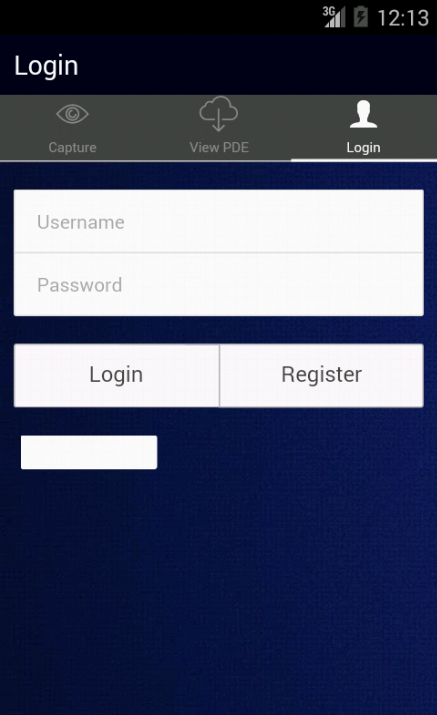
\includegraphics[width=50mm,scale=0.5]{images/screenshots/login.png}
\end{center}
\end{figure}
\begin{figure}[H]
\begin{center}
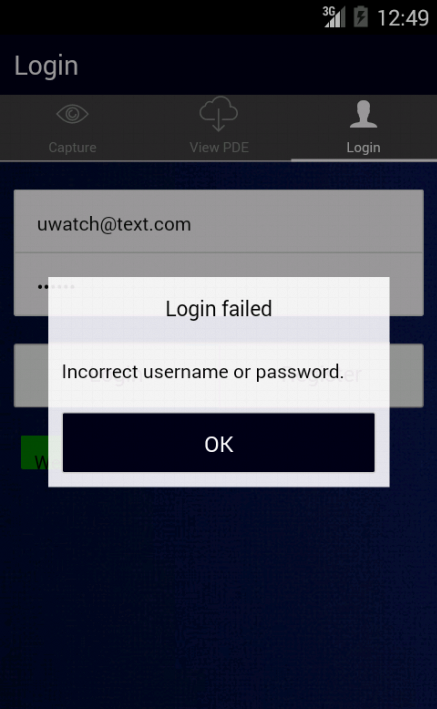
\includegraphics[width=50mm,scale=0.5]{images/screenshots/loginerror.png}
\end{center}
\end{figure}
\subsection{Capturing Potential Digital Evidence}
After you have logged in, click on the capture tab and the screen below will pop pup. Choose the type of media you want to use to capture your evidence by pressing the suitable button.
\begin{figure}[H]
\begin{center}
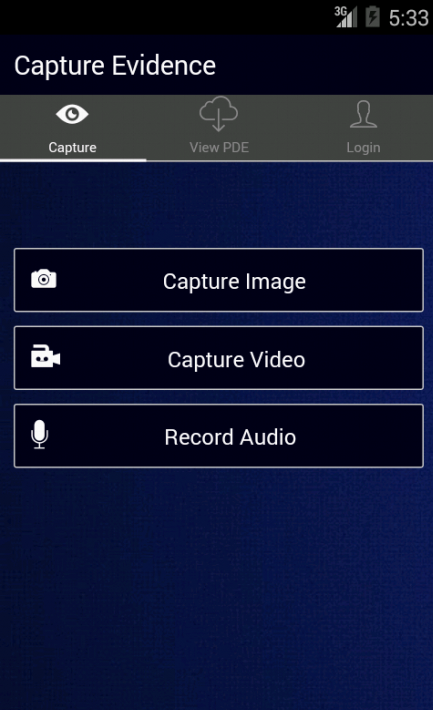
\includegraphics[width=50mm,scale=0.5]{images/screenshots/home.png}
\end{center}
\end{figure} 
Below is the example of how it looks when capturing an image.
\begin{figure}[H]
\begin{center}

\includegraphics[width=50mm,scale=0.5]{images/screenshots/captureimage.png}
\end{center}
\end{figure}
An example of how it looks when taking a video.
\begin{figure}[H]
\begin{center}
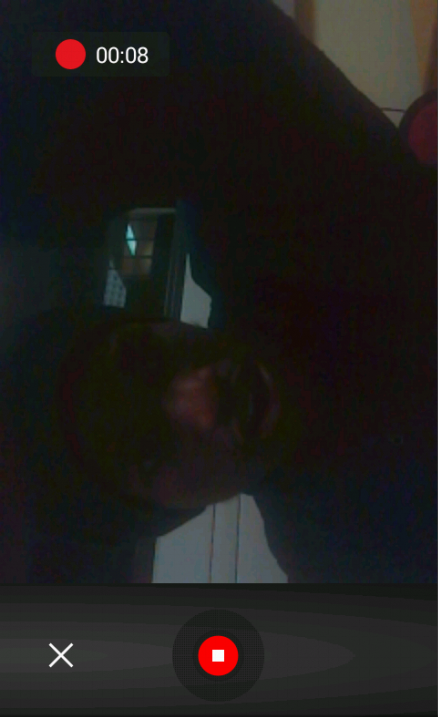
\includegraphics[width=50mm,scale=0.5]{images/screenshots/capturevideo.png}
\end{center}
\end{figure}
An example of how it looks when recording an audio.
\begin{figure}[H]
\begin{center}
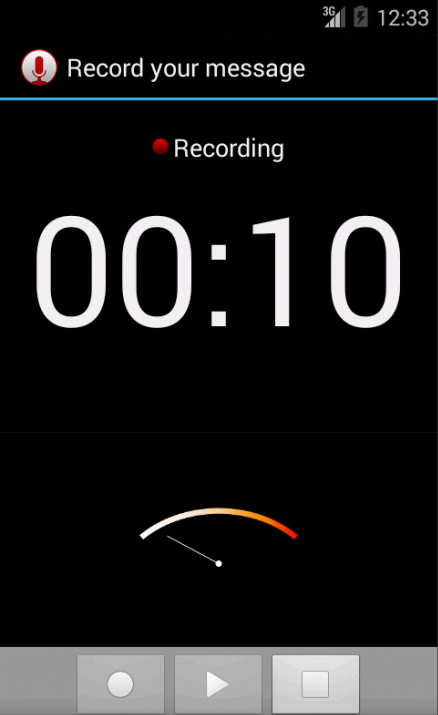
\includegraphics[width=50mm,scale=0.5]{images/screenshots/record.png}
\end{center}
\end{figure}
After you have captured your PDE you need to confirm that you are really uploading it by clicking ok button.
\begin{figure}[H]
\begin{center}
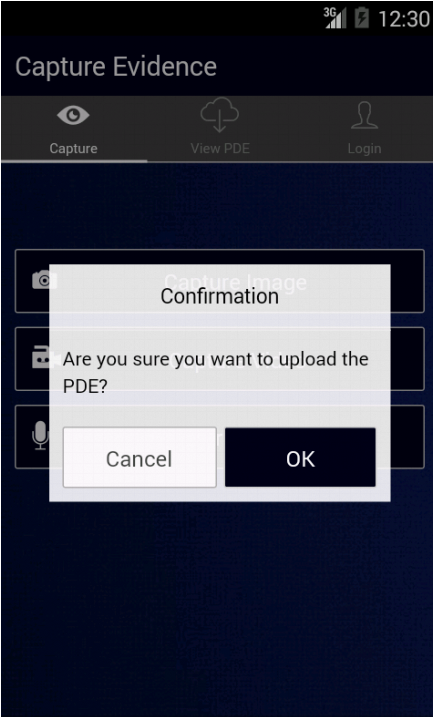
\includegraphics[width=50mm,scale=0.5]{images/screenshots/confirm.png}
\end{center}
\end{figure}
\begin{figure}[H]
\begin{center}
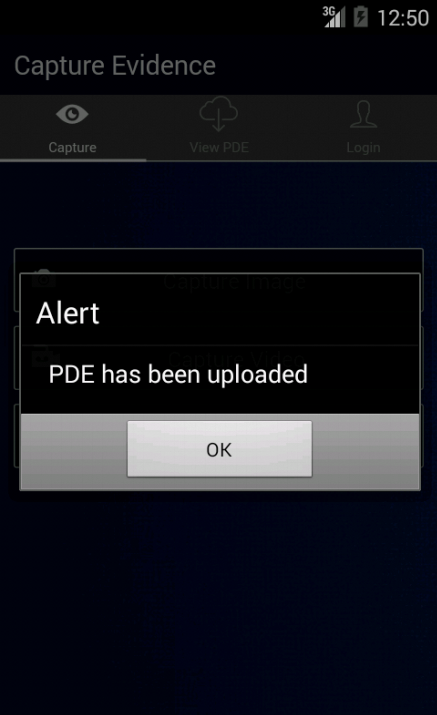
\includegraphics[width=50mm,scale=0.5]{images/screenshots/uploadsuccess.png}
\end{center}
\end{figure}
Or you can cancel the upload by clicking the cancel button.
\begin{figure}[H]
\begin{center}
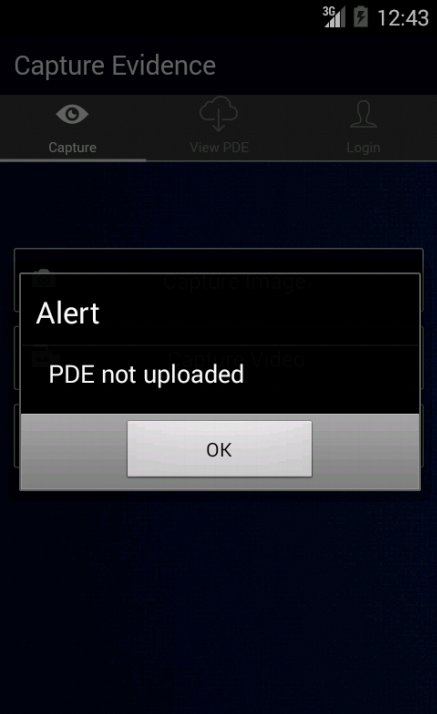
\includegraphics[width=50mm,scale=0.5]{images/screenshots/cancelcapture.png}
\end{center}
\end{figure}
\subsection{Viewing Potential Digital Evidence}
You can view your uploads by clicking on the view PDE tab after your uploads have succeeded.
\begin{figure}[H]
\begin{center}
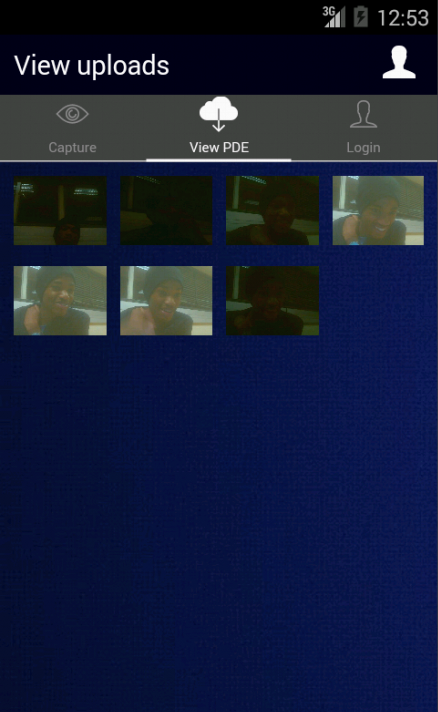
\includegraphics[width=50mm,scale=0.5]{images/screenshots/viewpde.png}
\end{center}
\end{figure}

\section{Troubleshooting}
Some evidence may not pass the test of authenticity, to fix this one should make use of more features of the app, for instance the location setting should be switched on and the camera should take high quality photos and videos. There will also be a problem if ones internet connection is not available, so the user should make sure of a stable connection to the internet when using the application. Other than that one should not have to troubleshoot.

\end{document}